\chapter{Versuchsdurchführung}

    \section{Charakterisierung des Cantilevers}

Zur Mikroskopierung einiger Proben wird in diesesm Versuch der dynamische Modus des
Mikroskops verwendet. Dies erfordert Kenntnis über das dynamische Verhalten des 
Cantilevers. Daher soll die Resonanzkurve aufgezeichnet und daraus die Güte der
Messspitze bestimmt werden. \par
\begin{figure}[hb]
    \centering
    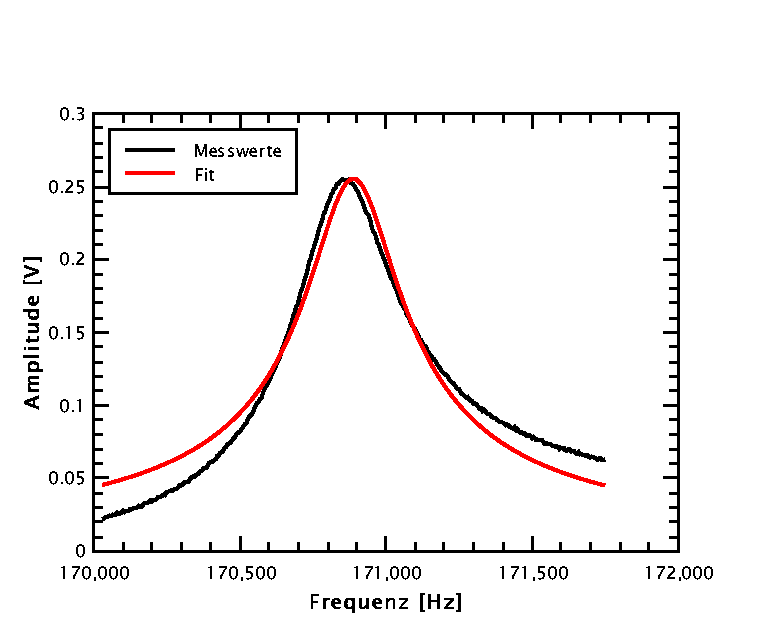
\includegraphics[width=0.6\textwidth]{Mess/freqsweep_2.pdf}
    \caption{Resonanzkurve des Cantilevers gefittet mit Gleichung des getriebenen,
             gedämpften Oszillators}
    \label{freqsweep}
\end{figure}
In Abbildung \ref{freqsweep} ist die aufgenommene Resonanzkurve zu sehen, gefittet
mit der Formel
\[
    A(\omega) = \frac{F_0}{m \sqrt{(\omega_0^2 - \omega^2)^2 + \left( 
    \frac{\omega\omega_0}{Q} \right)^2} }
\]
des getriebenen, gedämpften Oszillators. Aus dem Graphen lassen sich einige Werte
bestimmen, die im weiteren Verlauf des Versuches nützlich sein werden.
\begin{align*}
    Q=551,8 & & \frac{F_0}{m} = \SI{13,5}{MN\per\kg} & & \omega_0 =
    \SI{170,9}{kHz}
\end{align*}
Q bezeichnet hierbei den Gütefaktor des Cantilevers und $\omega_0$ die 
Resonanzfrequenz. \par
Anders als theoretisch errechnet, ist die gemessene Kurve nicht ganz symmetrisch.
Dies ist auf die Annäherung des Messkopfes als Massepunkt zurückzuführen. Die 
theoretische Betrachtung der räumlichen Ausdehnung würde zu höheren Termen führen,
die hier nicht näher betrachtet werden sollen.

    \section{Überprüfung der Geräteparameter}

Um Entfernungen auf Proben messen zu können, müssen die an den Piezo angelegten 
Spannungen zuverlässig in $x$, $y$ und $z$ Auslenkungen umgerechnet werden können.
Um diese Kalibrierung zu überprüfen, wird ein Eichgitter mit einer Gitterperiode
von  $\SI{10}{\mu m}$ verwendet.
\begin{figure}[hb]
    \centering
    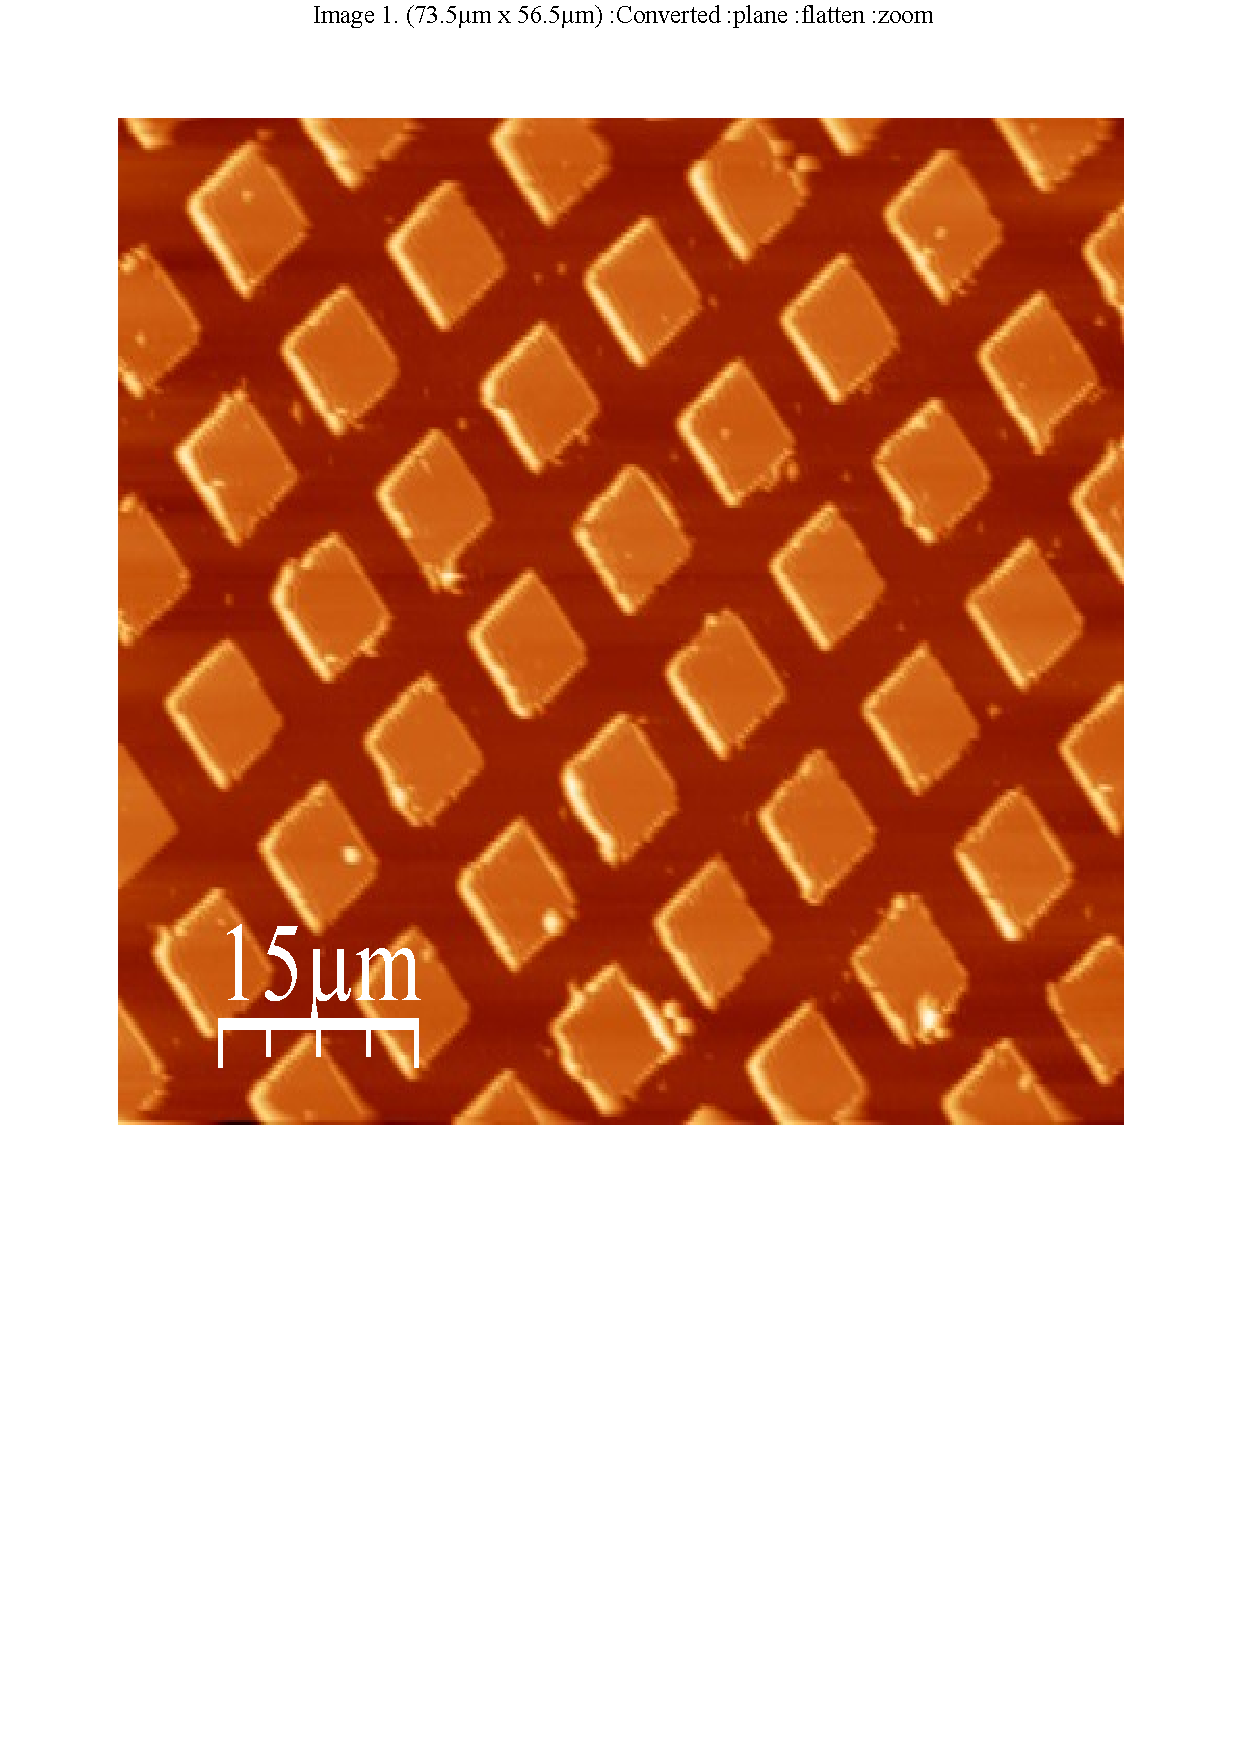
\includegraphics[width=0.4\textwidth]{Mess/gitter_aso.pdf}
    \caption{Mikroskopierung des Eichgitters}
    \label{gitter}
\end{figure}
In Abbildung \ref{gitter} ist eine Teilaufnahme des Gitters zu sehen. Der Abstand die 
zweier Quadrate beträgt laut Messung $\SI{10,06}{\mu m}$. Dies ist ein gutes 
Ergebnis, weshalb die Default-Werte im weiteren Verlauf des Versuch verwendet 
werden.

    \section{Spektroskopie}

Nun soll die Amplitude der oszillierenden Messspitze bestimmt werden. Hierzu wird
der Kopf über einer homogenen Oberfläche positioniert und die Änderung der 
Schwingungsamplitude bei Annäherung an die Probe aufgezeichnet.
\begin{figure}[hp]
    \centering
    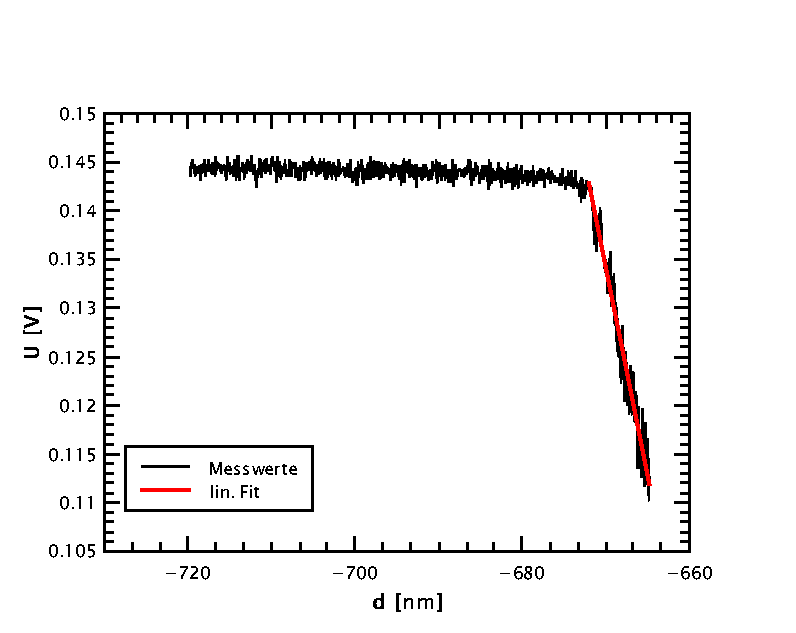
\includegraphics[width=0.6\textwidth]{Mess/spek_forw.pdf}
    \caption{Änderung der Amplitude bei Annäherung an Probe}
    \label{spek_forw}
\end{figure}
\begin{figure}[hp]
    \centering
    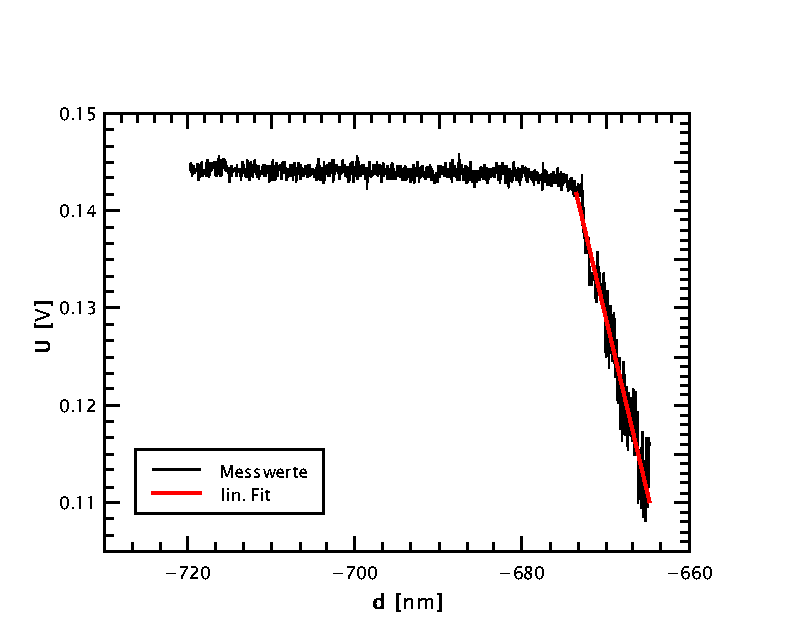
\includegraphics[width=0.6\textwidth]{Mess/spek_backw.pdf}
    \caption{Änderung der Amplitude bei Entfernung von Probe}
    \label{spek_backw}
\end{figure}
In den Abbildungen \ref{spek_forw} und \ref{spek_backw} sind diese Messungen, erst
bei Annäherung an die Probe, dann bei Entfernung von der Probe, zu sehen. Die 
Amplitude ist bei großen Entfernungen nahezu konstant. Bei Kontakt zwischen Spitze
und Probe befindet sich der untere Umkehrpunkt der Oszillation an der Probenfläche.
Somit sinkt die Amplitude um die Änderung der z-Position. Dieser lineare 
Zusammenhang zwischen Höhe des Cantilevers und der Amplitude soll nun zur 
Bestimmung der Amplitude benutzt werden.\par
Aus den linearen Fits kann die Proportionalitätskonstante für beide Messungen
bestimmt werden.
\begin{align*}
    K_{\text{for}} = \SI{4,27 \cdot 10^6}{A s \per N} & & K_{\text{rück}} = 
    \SI{5,61 \cdot 10^6}{A s \per N}
\end{align*}
Mithilfe der Formel $\displaystyle A = \frac{U}{K}$ und der Spannung vor Annäherung
an die Probe von $U \approx \SI{140}{mV}$ kann die Amplitude zu
\begin{align*}
    A = \frac{U}{K} \approx \frac{\SI{140}{mV}}{4,93 \cdot 10^6} = \SI{29,2}{nm}
\end{align*}
bestimmt werden.

    \section{Spur-Abstand einer CD}

Zuletzt soll mithilfe des Mikroskops die Kapazität einer CD bestimmt werden. Hierzu
soll die Spurbreite und der Bitabstand bestimmt werden, um die Fläche eines 
Datenpunktes zu errechnen. Kennt man die Fläche der CD, kann so auf die Kapazität 
geschlossen werden. \par
\begin{figure}[h]
    \centering
    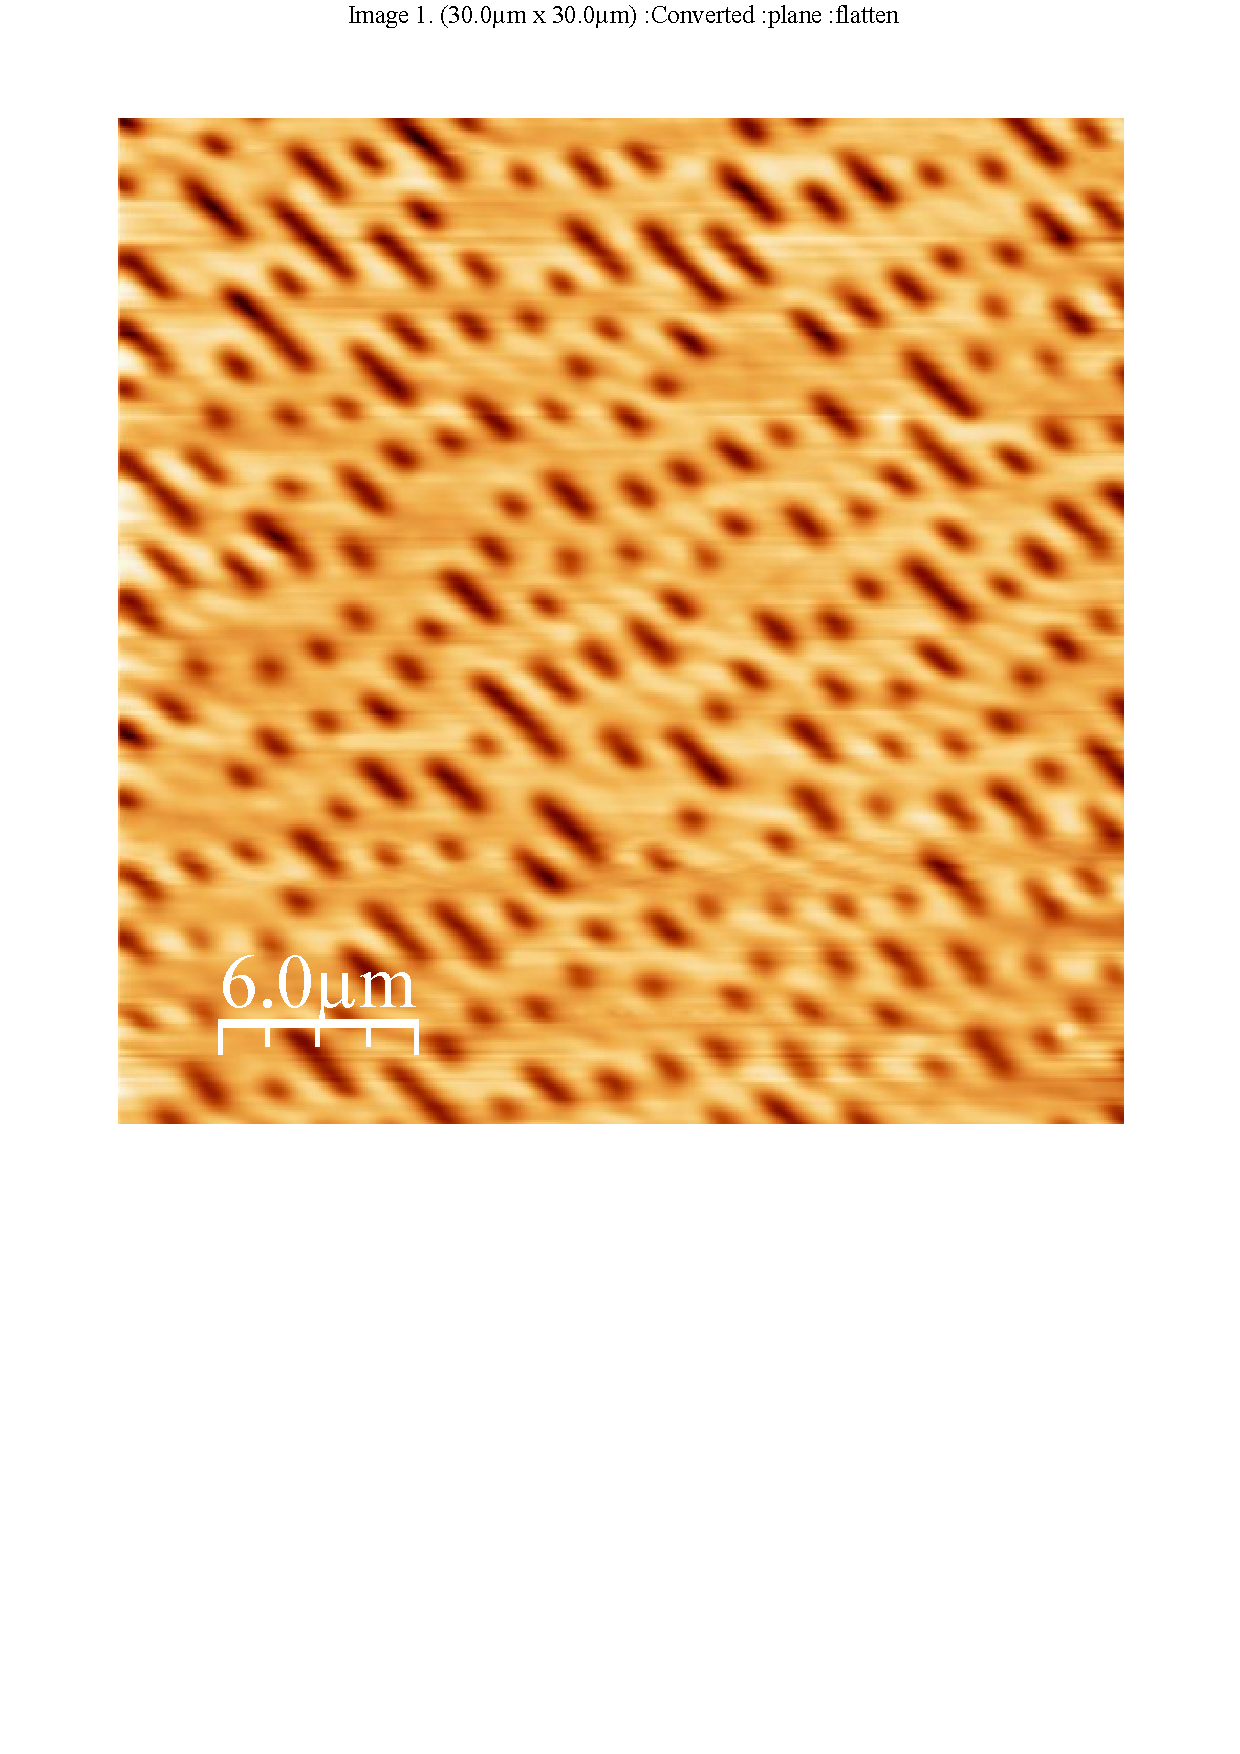
\includegraphics[width=0.4\textwidth]{Mess/cd.pdf}
    \caption{Mikroskopierung der Datenseite einer CD}
    \label{cd}
\end{figure}
Aus Abbildung \ref{cd} kann der Spurabstand zu $\SI{1,285}{\mu m}$ und der 
Bitabstand zu $\SI{1,250}{\mu m}$ bestimmt werden. Die Fläche eines Datenpunktes
beläuft sich somit auf $A_{Bit} = \SI{1,61}{\mu m^2}$. \par
Zur Bestimmung der beschreibbaren Fläche muss der Radius des ausgeschnittenen
Ringes von dem der CD abgezogen werden. 
\[
    A_{Data} = \pi \cdot \left( \underset{=\SI{58}{mm}}{\underbrace{r_{\text{außen}}^2}}
    - \underset{=\SI{25}{mm}}{\underbrace{r_{\text{innen}}^2 }} \right)
    = \SI{8604822000}{\mu m^2}
\]
Die Kapazität errechnet sich somit zu
\[
    N = \frac{A_{Data}}{A_{Bit}} \approx \SI{638}{MB}
\]
Der angegebene Wert ist $\SI{650}{MB}$. Die Abschätzung liefert somit ein gutes Ergebnis.
